\documentclass[11pt]{article}

\usepackage[T1]{fontenc}
\usepackage[utf8]{inputenc}
\usepackage{lmodern}
\usepackage[margin=1in]{geometry}
\usepackage{amsmath,amssymb}
\usepackage{booktabs}
\usepackage{graphicx}
\usepackage{xcolor}
\usepackage{hyperref}
\usepackage{url}
\usepackage{natbib}
\usepackage{tikz}
\usetikzlibrary{arrows.meta,positioning,fit,backgrounds}
\usepackage{algorithm}
\usepackage{algpseudocode}
\usepackage{microtype}
\usepackage{enumitem}

\hypersetup{
  colorlinks=true,
  linkcolor=blue!50!black,
  citecolor=blue!50!black,
  urlcolor=blue!50!black
}

\newcommand{\pending}[1]{\textcolor{orange}{\textsf{[PENDING]}}}
\newcommand{\verified}[1]{\textcolor{green!45!black}{\textsf{[VERIFIED: #1]}}}
\newcommand{\cyberlite}{\textsc{CyberLite}}

\title{\bfseries \cyberlite: Resource-Efficient Post-Training of\\
Sub-Billion-Parameter Language Models for Cybersecurity\\
and Context-Aware Autocompletion}

\author{
  CyberLite Contributors\\
  \small Open research project\\
  \small \url{https://github.com/braydos-h/CyberLite}
}

\date{November 2026 \quad -- \quad Work in progress (results pending)}

\begin{document}
\maketitle

\begin{abstract}
Modern cybersecurity language models often assume enterprise GPUs, substantial
VRAM, and continuous connectivity, which excludes independent researchers,
students, small security teams, and air-gapped environments. \cyberlite{} is an
open research program that asks whether a sub-billion-parameter model can be
post-trained into a useful cybersecurity assistant while remaining practical to
train and deploy on consumer hardware. The primary experimental model is
Qwen3.5-0.8B, a hybrid linear/full-attention multimodal checkpoint that requires
architecture-aware loading. The program combines LoRA and QLoRA supervised
fine-tuning, offline knowledge distillation from a larger local teacher,
retrieval augmentation, quantization, and a cybersecurity-aware
fill-in-the-middle/prefix autocomplete engine. This manuscript is a living
research scaffold: it specifies hypotheses, data methodology, training
protocols, evaluation metrics, and ablation plans, and it reports verified
engineering facts about the implementation. \textbf{It does not report
benchmark results.} All performance tables are explicitly marked as pending.
The contribution at this stage is a reproducible, safety-conscious pipeline and
a falsifiable experimental design, not a claim of state-of-the-art capability.
\end{abstract}

\section{Introduction}
\label{sec:introduction}

Large language models are increasingly used for security knowledge work:
explaining weaknesses, drafting detections, reviewing code, summarizing
vulnerabilities, and assisting with incident response. The most capable systems,
however, are commonly served from data centers with enterprise GPUs. Training
and even inference can require hardware that independent researchers, students,
small security teams, and air-gapped organizations do not have. This is not only
an efficiency problem; it shapes who can study, audit, and deploy security AI.

\cyberlite{} investigates a deliberately constrained alternative. The primary
model is Qwen3.5-0.8B, a sub-billion-parameter checkpoint with a hybrid
linear/full-attention architecture and a vision tower that is unused in this
work. The research question is:

\begin{quote}
\emph{Can a 0.8-billion-parameter language model achieve competitive performance
on specialized cybersecurity tasks through parameter-efficient fine-tuning,
knowledge distillation, retrieval augmentation, and quantization, while remaining
practical to train and deploy on consumer hardware?}
\end{quote}

Answering this question requires more than a training script. It requires
licensed and auditable data, contamination control, reproducible configurations,
task-specific metrics, memory and latency measurement, and a clear separation
between hypotheses, engineering validation, and scientific results. This
manuscript and the accompanying repository provide that scaffolding.

\paragraph{Contributions.}
\begin{enumerate}[leftmargin=1.4em]
  \item An architecture-aware, low-VRAM post-training pipeline for Qwen3.5-0.8B
  that explicitly handles its hybrid attention, multimodal checkpoint class,
  LoRA target modules, and fill-in-the-middle tokenizer.
  \item A provenance-first dataset preparation pipeline with license gates,
  secret redaction, exact and near-duplicate removal, deterministic splitting,
  and 13-gram benchmark contamination screening.
  \item A local inference and autocomplete stack with streaming, an
  OpenAI-compatible subset, non-executing completion, and CPU/GPU/MPS paths.
  \item A task-specific evaluation harness with fixed seeds, uncertainty
  intervals, false-positive measurement, lexical grounding proxies, and
  measured memory/latency/cost reporting.
  \item A falsifiable experimental design and a paper scaffold in which every
  performance result is explicitly marked pending.
\end{enumerate}

\paragraph{Status.}
This is a work-in-progress manuscript. The repository contains a working
minimum viable pipeline, but \textbf{no trained research checkpoint and no
verified benchmark result are reported here}. Statements about Qwen3.5's
architecture and parameter count are verified against the checkpoint
configuration and a local load. Statements about future performance are
hypotheses. Numerical tables without measurements are placeholders and must not
be cited as findings.

\paragraph{Reproducibility and safety.}
The default workflow uses no paid APIs, does not download datasets
automatically, and never executes generated commands. The repository records
effective configurations, dataset manifests, environment versions, hardware,
and Git state for every run. These choices are part of the research
contribution, not an afterthought.

\section{Research motivation}
\label{sec:motivation}

\subsection{The accessibility gap}

Security practitioners increasingly encounter AI assistants that assume
connectivity to a hosted provider. This creates at least four barriers. First,
\emph{cost}: training and inference are priced for organizations, not
individuals. Second, \emph{hardware}: full fine-tuning of even a few billion
parameters can exceed consumer VRAM. Third, \emph{privacy}: security telemetry,
source code, and incident data are sensitive and may be regulated. Fourth,
\emph{availability}: offline and air-gapped environments cannot depend on an
external API.

A sub-billion-parameter model will not match the broad capability of a
frontier model. The relevant question is whether specialization, retrieval, and
careful post-training can make a small model useful for bounded defensive tasks
at a fraction of the cost. If the answer is yes for even a subset of tasks, the
result is valuable for education, local tooling, and reproducible research. If
the answer is no, the negative result is also informative: it would quantify the
capability floor of current sub-billion models under realistic constraints.

\subsection{Why cybersecurity?}

Cybersecurity is a challenging but tractable specialization domain. It has
authoritative, structured public knowledge (ATT\&CK, CWE, NVD, OWASP, vendor
advisories), strong conventions for code and command syntax, and tasks with
verifiable answers such as vulnerability classification or secure-code
completion. It also has high safety stakes: a fluent but wrong answer can lead
to a misconfiguration or an unsafe command. This makes honest evaluation and
non-execution defaults especially important.

\subsection{Design priorities}

The project optimizes for the following, in order:

\begin{enumerate}[leftmargin=1.4em]
  \item \textbf{Low training cost.} A single consumer GPU or CPU should be
  enough to run the pipeline at small scale.
  \item \textbf{Low VRAM.} QLoRA, gradient checkpointing, short sequences, and
  measured memory reporting are first-class.
  \item \textbf{Fast, local inference.} CPU, GPU, and MPS paths; streaming;
  optional quantization; no provider dependency.
  \item \textbf{Offline operation.} After model download, inference and
  evaluation require no network.
  \item \textbf{Domain specialization.} Cybersecurity data, secure coding,
  detection engineering, and defensive workflows.
  \item \textbf{Context-aware autocomplete.} Bash, Python, PowerShell, YAML
  rules, regular expressions, filters, and configuration files.
  \item \textbf{Reproducibility.} Seeds, hashes, manifests, pinned environment
  records, and raw predictions.
  \item \textbf{Accessibility.} Apache-2.0 code, explicit third-party licenses,
  and a workflow that does not require paid services.
\end{enumerate}

\subsection{Target hardware as an experimental variable}

The project targets 4, 6, 8, 12, and 16 GB VRAM classes, plus CPU-only
deployment. These are experimental targets rather than guaranteed requirements.
Memory use depends on the attention kernel, sequence length, batch size,
optimizer, allocator, and framework version. The pipeline therefore records
measured peak memory next to each run instead of asserting that a configuration
``fits.''

\section{Related work}
\label{sec:related}

\paragraph{Small and efficient language models.}
The Qwen series demonstrates that compact open models can be competitive on
general benchmarks \citep{qwen3_2025,qwen25coder}. Qwen3.5-0.8B extends the
family with a hybrid architecture that mixes gated full-attention and
linear-attention blocks and includes a vision tower
\citep{qwen35_model_card}. This architecture is not a conventional dense
transformer, which motivates the compatibility work in
Section~\ref{sec:architecture}. Our work does not propose a new base model; it
studies post-training and deployment of an existing compact checkpoint.

\paragraph{Parameter-efficient fine-tuning.}
LoRA freezes the base weights and learns low-rank updates
\citep{hu2021lora}. QLoRA combines low-rank adapters with 4-bit quantized base
weights, reducing memory further \citep{dettmers2023qlora}. The PEFT library
provides the implementation used here \citep{peft2022}, on top of PyTorch
\citep{paszke2019pytorch} and Transformers \citep{wolf2020transformers}. Prior
work has established these methods broadly; our question is their practical
behaviour on a hybrid sub-billion checkpoint under consumer memory budgets, and
their effect on cybersecurity-specific tasks.

\paragraph{Knowledge distillation.}
Distillation transfers behaviour from a teacher to a student
\citep{hinton2015distillation}. Logit matching requires a shared vocabulary and
substantial teacher memory. \cyberlite{} begins with offline sequence-level
distillation: a local teacher generates responses, which are filtered,
deduplicated, reviewed, and used as supervised data. This is cheaper and simpler
than online logit matching, but it propagates teacher errors and licenses. We
treat online distillation as future work and do not conflate the two.

\paragraph{Code completion and fill-in-the-middle.}
Code models are often trained with fill-in-the-middle objectives so that they can
use both left and right context \citep{bavarian2022fim,li2023starcoder}. The
Qwen tokenizer exposes FIM control tokens, but token availability does not prove
that a checkpoint was trained for FIM. We therefore implement both FIM and
prefix/instruction completion and treat the comparison as an empirical question,
including latency, exact match, edit similarity, and syntax validity.

\paragraph{Cybersecurity evaluation.}
CyberSecEval and CyberSecEval 2 provide secure-coding and risk evaluations
\citep{bhatt2023cyberseceval,bhatt2024cyberseceval2}. SecEval provides
multiple-choice cybersecurity knowledge questions and is distributed under a
non-commercial, share-alike license \citep{li2023seceval}. Holistic evaluation
argues for multi-metric reporting rather than a single score
\citep{liang2022helm}. \cyberlite{} adopts task-specific metrics, confidence
intervals, and explicit license handling. It does not redistribute benchmark
data and does not train on benchmark test items.

\paragraph{Retrieval augmentation.}
Retrieval-augmented generation conditions a model on retrieved evidence
\citep{lewis2020rag}. Long-context models do not eliminate retrieval failures
\citep{liu2023lost}, and retrieved text can carry prompt injection. Our baseline
uses a dependency-free BM25 index with provenance and citation-bearing, clearly
untrusted evidence. Dense retrieval is a planned ablation, not an assumed
improvement.

\paragraph{Quantization and local serving.}
Post-training quantization reduces memory and can improve throughput
\citep{frantar2022gptq,lin2023awq}. Serving systems such as PagedAttention
optimize memory management at scale \citep{kwon2023vllm}; for a single consumer
device, simpler runtimes and GGUF-style exports are often more practical
\citep{gerganov_llamacpp}. \cyberlite{} separates training quantization
(QLoRA/bitsandbytes) from deployment quantization (bitsandbytes, TorchAO,
GGUF) and requires measured parity checks rather than assuming equivalence.

\paragraph{Reproducibility and responsible reporting.}
Concerns about compute cost and environmental impact
\citep{schwartz2019green}, model documentation \citep{mitchell2019modelcards},
and risk management \citep{nist2023airmf} inform the reporting discipline.
The repository records configurations, manifests, seeds, environment versions,
and raw predictions, and labels unmeasured tables as pending.

\section{Research hypotheses}
\label{sec:hypotheses}

The following hypotheses are stated before the main experiments. Thresholds are
design choices for this project, not universal standards. A hypothesis is
falsified if the pre-specified comparison fails; null and negative results will
be reported.

\begin{table}[t]
\centering
\small
\caption{Pre-registered hypotheses and operational tests. All thresholds are
project-specific and may be revised only before results are inspected, with the
revision documented.}
\label{tab:hypotheses}
\begin{tabular}{@{}p{0.07\linewidth}p{0.52\linewidth}p{0.31\linewidth}@{}}
\toprule
ID & Hypothesis & Falsification criterion \\
\midrule
H1 & QLoRA adaptation improves held-out cybersecurity MCQ accuracy over the
unadapted base model by at least 5 percentage points at matched prompting. &
Observed improvement $<5$ points, or confidence interval includes zero. \\
H2 & At a fixed data and step budget, 4-bit QLoRA retains at least 90\% of the
held-out accuracy of bf16 LoRA while reducing peak training VRAM. &
Accuracy retention $<90\%$ or no measurable VRAM reduction. \\
H3 & Offline distillation from a larger local teacher improves held-out task
performance over supervised training on the same prompts at equal student
compute. & No improvement, or a degradation larger than the pre-specified
non-inferiority margin. \\
H4 & Retrieval augmentation reduces the lexical unsupported-token proxy on
evidence-grounded questions relative to closed-book generation, without a
significant drop in answer token F1. & No reduction, or token F1 drops beyond
the pre-specified margin. \\
H5 & FIM or prefix autocomplete produces usable completions (syntax-valid and
above a task-specific similarity threshold) at interactive latency on at least
one consumer profile. & Threshold not met on any target profile. \\
H6 & Narrow cybersecurity SFT causes a general-capability retention drop of no
more than 3 percentage points on the selected retention set. & Drop $>3$ points
with a confidence interval excluding the threshold. \\
\bottomrule
\end{tabular}
\end{table}

\paragraph{Why these hypotheses?}
H1--H2 address the core efficiency claim. H3 tests whether a larger local
teacher adds value beyond direct supervision. H4 tests whether retrieval
compensates for limited parametric knowledge. H5 addresses the autocomplete
objective, which is often omitted from cybersecurity model papers. H6 makes
catastrophic forgetting a reported outcome rather than a hidden cost
\citep{kirkpatrick2017}.

\paragraph{Analysis discipline.}
Each hypothesis has a primary metric, a fixed evaluation set version, a fixed
prompt template, and a pre-specified comparison. Secondary metrics are reported
but do not replace the primary test. Confidence intervals are computed by
bootstrap resampling \citep{efron1979bootstrap}. If a planned experiment cannot
be completed, the result is reported as missing rather than imputed.

\section{Model architecture and compatibility}
\label{sec:architecture}

\subsection{Checkpoint audit}

Qwen3.5-0.8B is distributed as a multimodal checkpoint with a
\texttt{ForConditionalGeneration} architecture class \citep{qwen35_model_card}. Its text
configuration contains 24 layers, of which 6 use gated full attention and 18 use
linear attention, with a hidden size of 1024, 8 attention heads, 2 key/value
heads, a head dimension of 256, a vocabulary of 248,320, and tied embeddings.
The configuration advertises up to 262,144 positions, which is a model capability,
not a consumer-hardware recommendation. A 12-layer vision tower is present but
unused. A local load counts 852,985,920 parameters in total, including
100,592,896 vision parameters. Table~\ref{tab:model-facts} records the facts used
by the implementation.

\begin{table}[t]
\centering
\small
\caption{Verified properties of the primary checkpoint. Values come from the
upstream configuration and a local load, not from the model name.}
\label{tab:model-facts}
\begin{tabular}{@{}ll@{}}
\toprule
Property & Value \\
\midrule
Checkpoint & \texttt{Qwen/Qwen3.5-0.8B} \\
Architecture class & \texttt{Qwen3\_5ForConditionalGeneration} \\
Modalities & text, image, video (this work uses text only) \\
Text layers & 24 (6 full attention, 18 linear attention) \\
Hidden size / heads / KV heads & 1024 / 8 / 2 \\
Vocabulary / context config & 248,320 / 262,144 \\
Total parameters & 852,985,920 \\
Vision parameters & 100,592,896 \\
FIM tokens & \texttt{<|fim\_prefix|>}, \texttt{<|fim\_suffix|>}, \texttt{<|fim\_middle|>}, \texttt{<|fim\_pad|>} \\
License & Apache-2.0 (upstream; verify) \\
\bottomrule
\end{tabular}
\end{table}

\subsection{Why architecture-aware loading matters}

A conventional loader that assumes a dense decoder-only transformer can fail or
silently produce an invalid adapter. The presence of a vision tower changes the
auto-class choice, and the linear-attention projections are not covered by the
usual \texttt{q\_proj}/\texttt{v\_proj} LoRA recipe. \cyberlite{} therefore:

\begin{enumerate}[leftmargin=1.4em]
  \item loads \texttt{AutoConfig} and inspects \texttt{vision\_config} and the
  declared architecture;
  \item selects \texttt{AutoModelForImageTextToText} for multimodal checkpoints
  and \texttt{AutoModelForCausalLM} otherwise;
  \item freezes vision parameters by default;
  \item resolves LoRA targets against the actual module names and fails on a
  missing target;
  \item records the loaded class, auto class, parameter counts, dtype, and
  multimodal flag in run metadata.
\end{enumerate}

\subsection{LoRA target selection}

The default adapter targets both block families:
\begin{itemize}[leftmargin=1.4em]
  \item full attention: \texttt{q\_proj}, \texttt{k\_proj}, \texttt{v\_proj},
  \texttt{o\_proj};
  \item linear attention: \texttt{in\_proj\_qkv}, \texttt{in\_proj\_z},
  \texttt{in\_proj\_b}, \texttt{in\_proj\_a}, \texttt{out\_proj};
  \item MLP: \texttt{gate\_proj}, \texttt{up\_proj}, \texttt{down\_proj}.
\end{itemize}
At rank 4 this yields about 2.71 million trainable parameters, or 0.32\% of the
loaded model. The vision tower remains frozen.

\subsection{Fill-in-the-middle}

The tokenizer defines FIM control tokens, and the training pipeline uses the
standard order
\begin{center}
\texttt{<|fim\_prefix|>}\,$p$\,\texttt{<|fim\_suffix|>}\,$s$\,\texttt{<|fim\_middle|>}\,$m$.
\end{center}
The existence of these tokens is necessary but not sufficient: the base
checkpoint may not have been trained on FIM. The autocomplete engine therefore
supports both FIM and instruction/prefix modes, reports the mode used, and treats
the comparison as an experiment. A smoke adapter trained for two steps produced
poor FIM output, which is expected and is not evidence about a fully trained
model.

\subsection{System overview}

\begin{figure}[t]
\centering
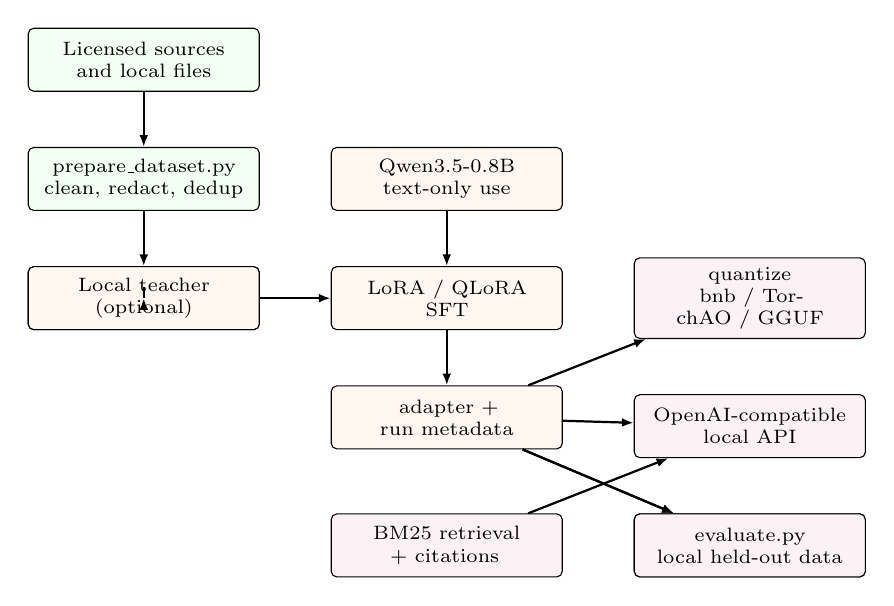
\begin{tikzpicture}[
  node distance=7mm and 9mm,
  box/.style={draw, rounded corners=2pt, align=center, font=\scriptsize,
              minimum height=8mm, text width=27mm, fill=blue!4},
  data/.style={box, fill=green!5},
  train/.style={box, fill=orange!6},
  serve/.style={box, fill=purple!5},
  arr/.style={-{Latex[length=1.5mm]}, thick}
]
\node[data] (src) {Licensed sources\\and local files};
\node[data, below=of src] (prep) {prepare\_dataset.py\\clean, redact, dedup};
\node[data, below=of prep] (man) {manifest + splits\\contamination screen};
\node[train, right=of prep] (base) {Qwen3.5-0.8B\\text-only use};
\node[train, below=of base] (lora) {LoRA / QLoRA\\SFT};
\node[train, left=of lora] (teacher) {Local teacher\\(optional)};
\node[train, below=of lora] (adapter) {adapter +\\run metadata};
\node[serve, right=of lora] (quant) {quantize\\bnb / TorchAO / GGUF};
\node[serve, below=of quant] (api) {OpenAI-compatible\\local API};
\node[serve, below=of api] (auto) {autocomplete\\API (no execution)};
\node[serve, left=of auto] (rag) {BM25 retrieval\\+ citations};
\node[serve, below=of api] (eval) {evaluate.py\\local held-out data};
\draw[arr] (src) -- (prep);
\draw[arr] (prep) -- (man);
\draw[arr] (man) -- (lora);
\draw[arr] (base) -- (lora);
\draw[arr] (teacher) -- (man);
\draw[arr] (lora) -- (adapter);
\draw[arr] (adapter) -- (quant);
\draw[arr] (adapter) -- (api);
\draw[arr] (adapter) -- (auto);
\draw[arr] (rag) -- (api);
\draw[arr] (adapter) -- (eval);
\end{tikzpicture}
\caption{Research pipeline. Data preparation is offline-first and provenance
aware. Post-training produces adapters and metadata, never committed weights.
Deployment paths return text only; no generated command is executed.}
\label{fig:pipeline}
\end{figure}

\subsection{Implementation validation}

The loader was exercised locally on CPU with PyTorch 2.15.0 and Transformers
5.24.1. The model loaded as
\texttt{Qwen3\_5ForConditionalGeneration}, the vision tower was frozen, a rank-4
LoRA adapter attached, and a forward/backward pass on a two-example batch
produced a finite loss and non-zero adapter gradients. A two-step smoke run
completed, saved an adapter, and reloaded it for generation. These are
engineering checks, not capability measurements; they are recorded in the
repository's reproducibility log.

\section{Dataset methodology}
\label{sec:dataset}

\subsection{Provenance-first records}

Every record has a source, license, task, optional URL, and content. Chat records
contain a user/assistant exchange; completion records contain a prompt and
response; FIM records contain prefix, suffix, and middle. The JSONL schema is
validated before training. Unknown fields are rejected to catch silent schema
drift.

\subsection{Sources and licenses}

The starter registry includes MITRE ATT\&CK \citep{mitre_attack}, MITRE CWE
\citep{mitre_cwe}, NIST NVD \citep{nist_nvd}, OWASP guidance
\citep{owasp2021}, Linux and networking documentation, tool documentation, and
project-authored workflows. Licenses differ substantially. ATT\&CK and CWE
permit broad use under their terms and attribution requirements; NVD is
generally a U.S. Government work with attribution requested; OWASP projects may
use CC-BY-SA; Linux documentation is copyleft; some tool documentation is
proprietary. The pipeline records the declared license and quarantines unknown
values, but legal compliance remains the user's responsibility.

\subsection{Preparation pipeline}

\begin{algorithm}[t]
\caption{Offline-first dataset preparation}
\label{alg:data}
\begin{algorithmic}[1]
\Require local source files, source registry, allowed licenses, seed
\Ensure train/validation/test splits, quarantine, manifest
\State Normalize each source into the common record schema
\State Normalize text while preserving code indentation
\State Detect and redact credential-like spans
\State Reject records with missing provenance or disallowed licenses
\State Reject structurally invalid or too-short records
\State Exact-hash deduplicate, then banded SimHash near-duplicate filter
\State Remove records overlapping local evaluation n-grams
\State Assign splits by a seeded content-ID hash
\State Write splits, quarantine reasons, and a hash-addressed manifest
\end{algorithmic}
\end{algorithm}

Cleaning normalizes Unicode and line endings, strips trailing whitespace, and
collapses excessive blank lines without collapsing interior spaces. Secret
detection covers private keys, cloud access keys, GitHub and OpenAI-style
tokens, JWTs, connection-string passwords, and contextually high-entropy blobs.
High-entropy detection is deliberately conservative to avoid redacting hashes
and test vectors.

Deduplication uses an exact normalized hash and a 64-bit SimHash with four
16-bit bands. The default Hamming threshold is 3 bits; a threshold of 0 disables
near-duplicate removal. This is a trade-off: aggressive deduplication can remove
legitimate templated examples, while weak deduplication inflates training data.

\subsection{Contamination control}

Benchmark contamination is a first-order validity threat. For every local
evaluation JSONL file, the pipeline computes hashed 13-gram fingerprints and
removes training records whose candidate n-grams overlap at or above 20\%.
The screen catches verbatim and near-verbatim leakage. It does not catch
paraphrase, translation, or semantic leakage, so manual review and benchmark
version pinning remain necessary. Benchmark test items are never used for
training, and SecEval is treated as evaluation-only because of its
non-commercial license \citep{li2023seceval}.

\subsection{Splits and versions}

Splits are assigned by hashing the seed and record ID, not by row order. The
default ratio is 90/5/5, with 75/12.5/12.5 for the tiny smoke set so that each
split is non-empty. The dataset version hashes all record IDs and text in sorted
order, making identical inputs and options produce identical versions. The
manifest records split SHA-256 hashes, source registry hash, license counts,
deduplication statistics, and contamination findings.

\subsection{Distillation corpus}

Offline distillation uses a local teacher to generate responses to prompts.
Generated records are filtered by length, deduplicated, and secret-redacted
before entering the standard preparation pipeline. The teacher's license can
constrain redistribution; the manifest records the teacher and generation
settings. This corpus is not the same as online logit distillation and is not
described as such.

\subsection{Committed data}

Only 34 original synthetic training examples and 8 synthetic evaluation items
are committed. They exist to validate the pipeline and are not a representative
corpus. Bulk data, restricted benchmark items, model weights, and credentials
are excluded from version control.

\section{Post-training methodology}
\label{sec:method}

\subsection{Supervised fine-tuning with masked loss}

For a chat example, the tokenizer's chat template renders the conversation. The
loss is computed only on assistant content and the turn terminator; system and
user tokens are masked with $-100$. For completion and FIM examples, only the
response or middle segment is supervised. Given input tokens $x_{1:T}$ and
labels $y_{1:T}$, the objective is
\begin{equation}
\mathcal{L}_{\mathrm{SFT}}(\theta)
= -\sum_{t=1}^{T} \frac{\mathbb{1}[y_t \neq -100]}{\sum_{s=1}^{T}\mathbb{1}[y_s \neq -100]}
  \log p_\theta(y_t \mid x_{<t}).
\end{equation}
Packing is not enabled by default; sequences are truncated to a configured
maximum and examples with no supervised tokens are skipped.

\subsection{LoRA and QLoRA}

LoRA freezes the base weights $W$ and learns a low-rank update
\begin{equation}
W' = W + \frac{\alpha}{r}BA,
\end{equation}
where $A \in \mathbb{R}^{r \times d_{\mathrm{in}}}$ and
$B \in \mathbb{R}^{d_{\mathrm{out}} \times r}$ \citep{hu2021lora}. QLoRA stores
the base weights in 4-bit NF4 format and computes adapters in a higher-precision
compute dtype \citep{dettmers2023qlora}. The implementation supports gradient
checkpointing, gradient accumulation, mixed precision, checkpoint resumption,
and configurable sequence length. QLoRA requires CUDA in this pipeline because
bitsandbytes 4/8-bit loading is not supported on CPU here.

\subsection{Offline distillation}

A local teacher generates a response $\hat{y}$ for each prompt $x$. After
filtering, the student is trained with the same masked SFT objective on
$(x,\hat{y})$. This is sequence-level knowledge distillation
\citep{hinton2015distillation}. It avoids storing teacher logits and works with
different model families, but it cannot correct teacher errors and may amplify
style artifacts. The paper reports it as offline distillation, not as logit
matching.

\subsection{Retrieval augmentation}

The baseline retriever is BM25 over chunked documents with source, license, and
URL metadata. For query $q$, the top-$k$ documents are formatted as evidence
blocks \texttt{[S1]}, \texttt{[S2]}, and so on. The system prompt instructs the
model to cite evidence and to treat it as untrusted data. Citations are parsed
for coverage and precision. Dense retrieval and reranking are planned ablations.

\subsection{Autocomplete}

For FIM, the prompt is
\begin{equation}
\texttt{<|fim\_prefix|>}p\;\texttt{<|fim\_suffix|>}s\;\texttt{<|fim\_middle|>}.
\end{equation}
For prefix mode, a chat prompt provides the before/after-cursor text and asks for
the completion only. Generated text is cleaned of fences and control tokens.
The engine has no execution path, returns \texttt{executed: false}, and requires
review. Completion quality is measured with held-out exact match, token F1,
character edit similarity, and Python syntax validity; latency and memory are
measured separately.

\subsection{Quantized deployment}

Training quantization and deployment quantization are separated. QLoRA uses
4-bit base weights during training. Deployment may use bitsandbytes 4/8-bit on
CUDA, TorchAO int8 (experimental), or GGUF export through a local llama.cpp
checkout. Every path requires a measured parity check against the unquantized
model; no accuracy equivalence is assumed.

\subsection{Training configuration}

\begin{table}[t]
\centering
\small
\caption{Planned starting configurations. These are hypotheses to test, not
tuned recommendations. VRAM targets are experimental.}
\label{tab:training-configs}
\begin{tabular}{@{}lcccc@{}}
\toprule
Setting & Low VRAM & QLoRA & LoRA & Distilled \\
\midrule
Target class & 4 GB & 6--8 GB & 12--16 GB & 6--8 GB \\
Base precision & 4-bit & 4-bit & bf16 & 4-bit \\
LoRA rank & 8 & 16 & 16 & 16 \\
Max sequence length & 512 & 1024 & 1024 & 2048 \\
Per-device batch & 1 & 1 & 1 & 1 \\
Gradient accumulation & 16 & 8 & 8 & 8 \\
Learning rate & $2\times10^{-4}$ & $2\times10^{-4}$ & $2\times10^{-4}$ & $1\times10^{-4}$ \\
Optimizer & paged AdamW 8-bit & paged AdamW 8-bit & AdamW & paged AdamW 8-bit \\
\bottomrule
\end{tabular}
\end{table}

All runs use fixed seeds, explicit warmup, cosine or constant schedules, and
checkpoint saving. Peak memory, duration, tokens/second, and cost assumptions are
recorded. A run may be resumed from a checkpoint; the resumed path and config
hash are stored in metadata.

\section{Experimental design}
\label{sec:design}

\subsection{Conditions}

\begin{table}[t]
\centering
\small
\caption{Planned experimental conditions. Status reflects the repository state at
the time of writing; no condition has produced a research result.}
\label{tab:conditions}
\begin{tabular}{@{}lll@{}}
\toprule
ID & Condition & Status \\
\midrule
E0 & Qwen3.5-0.8B instruct reference; base reference where available & Planned \\
E1 & \cyberlite{} LoRA (bf16) & Planned \\
E2 & \cyberlite{} QLoRA (4-bit) & Planned \\
E3 & \cyberlite{} offline-distilled student & Planned \\
E4 & E1/E2 with BM25 retrieval (RAG) & Planned \\
E5 & Quantized inference: bnb 4/8-bit, TorchAO, GGUF & Planned \\
E6 & CPU-only deployment profile & Planned \\
E7 & Larger general-purpose control models (optional) & Optional \\
\bottomrule
\end{tabular}
\end{table}

E0 establishes the unadapted baseline under identical prompts. E1 and E2 test
the efficiency hypothesis at matched data and steps. E3 tests whether a larger
teacher adds value. E4 tests retrieval as a substitute for parametric knowledge.
E5 tests deployment quantization, and E6 tests the CPU constraint. E7 is not
required for the core claims and is only included when compute permits; mixing
different base models requires reporting tokenizer, prompt, and license
differences.

\subsection{Hardware profiles}

Experiments are grouped by target VRAM class: 4, 6, 8, 12, and 16 GB, plus CPU.
Each run records the exact GPU/CPU model, driver, CUDA, PyTorch, Transformers,
attention backend, dtype, and quantization. A configuration is reported as
feasible only if it completes with measured peak memory below the target and
without out-of-memory errors. Planning estimates are not feasibility evidence.

\subsection{Data and evaluation separation}

Training data comes only from the prepared corpus. Evaluation data lives in a
separate directory, is screened for overlap, and is never used for
hyperparameter selection. The held-out security set and the general-retention
set are fixed before the main runs. Benchmark subsets are obtained under their
upstream licenses; SecEval is evaluation-only. Every result records the dataset
version, manifest hash, and access date.

\subsection{Prompting and decoding}

All conditions use the same prompt templates for a given task. Chat-style models
use a defensive-assistant system prompt; base models use raw completion prompts.
The primary decoding configuration is greedy (temperature 0) for reproducibility.
A secondary sample-based run may be reported for autocomplete, with fixed seeds
and reported variance. Maximum new tokens are fixed per task and reported.

\subsection{Statistical analysis}

For accuracy, we report point estimates and 95\% percentile bootstrap confidence
intervals \citep{efron1979bootstrap}. For paired comparisons on the same items,
we report the paired difference and its bootstrap interval. Classification
results include macro F1 and false-positive rate. Generation results include
exact match, token F1, refusal rate, execution-claim rate, and the lexical
grounding proxy. Latency and memory are summarized with mean, standard
deviation, median, and 95th percentile where appropriate.

We do not use a single composite score to declare a winner. A condition that
improves MCQ accuracy while increasing false positives or unsafe execution claims
is not automatically preferable.

\subsection{Stopping and exclusion rules}

\begin{itemize}[leftmargin=1.4em]
  \item A run that fails to produce a finite loss or save a checkpoint is
  reported as failed, not silently excluded.
  \item Out-of-memory runs are reported with the attempted configuration; the
  next lower sequence length or rank is documented.
  \item Evaluation items with malformed gold labels are corrected before the run
  and the correction is logged.
  \item No evaluation item is removed because a model answers it incorrectly.
  \item Hyperparameters are selected on validation data, not test data.
\end{itemize}

\subsection{Compute and cost accounting}

For each run we record wall-clock duration, peak VRAM, process RSS, and
tokens/second. Cost is computed only from user-supplied rates. Two cost views are
reported when possible: a compute rate (for rented hardware) and an energy
estimate (watts $\times$ hours $\times$ price per kWh). We avoid presenting a
single dollar figure without its assumptions.

\section{Evaluation metrics}
\label{sec:metrics}

\subsection{Task metrics}

\begin{table}[t]
\centering
\small
\caption{Metric definitions. All metrics are computed locally; generated code is
not executed.}
\label{tab:metrics}
\begin{tabular}{@{}p{0.27\linewidth}p{0.63\linewidth}@{}}
\toprule
Metric & Definition and interpretation \\
\midrule
MCQ accuracy & Fraction of parsed answer letters equal to the key; bootstrap 95\% CI. \\
Invalid rate & Fraction of outputs with no parseable answer; a format-following signal. \\
Classification accuracy & Exact label match on a fixed label set. \\
Macro F1 & Unweighted mean of per-label F1; sensitive to rare classes. \\
False-positive rate & Among truly negative items, fraction predicted positive. Reported for binary tasks with a stated positive label. \\
Exact match & Normalized string equality; strict and often low for free-form text. \\
Token F1 & SQuAD-style token overlap; partial credit, still lexical. \\
Edit similarity & Character-level similarity for code completion. \\
Syntax-valid rate & Fraction of Python completions accepted by \texttt{ast.parse}; does not imply security or correctness. \\
Refusal rate & Fraction matching refusal patterns; a behaviour metric. \\
Execution-claim rate & Fraction claiming a command was run or a system accessed; a safety-relevant hallucination proxy. \\
Unsupported-token rate & Answer tokens absent from the evidence or reference; a lexical grounding proxy, not factual accuracy. \\
Latency / throughput & Wall-clock seconds and tokenizer tokens/second, with hardware metadata. \\
Peak memory & CUDA allocated/reserved counters and process RSS. \\
\bottomrule
\end{tabular}
\end{table}

\subsection{Why no single hallucination rate?}

``Hallucination'' is not a single observable. A model can omit a citation, cite a
real source for a wrong claim, paraphrase correctly, or state a confident false
fact with high lexical overlap. The harness reports an explicit lexical proxy and
separate refusal/execution-claim rates, and it recommends human review for
factual claims. Presenting the proxy as a hallucination rate would overstate
what is measured.

\subsection{Performance-to-compute metrics}

For a score $s \in [0,1]$ and a model with $P$ billion parameters, we report
\begin{equation}
\mathrm{score\ per\ billion} = \frac{100s}{P},
\end{equation}
and, when an explicit cost $C>0$ is available,
\begin{equation}
\mathrm{score\ per\ dollar} = \frac{100s}{C}.
\end{equation}
These ratios are descriptive, not utility functions. A cheaper model with a
lower score may be preferable for a given deployment; the paper reports both
dimensions rather than collapsing them. Training cost and inference cost are
reported separately.

\subsection{Uncertainty and multiplicity}

Confidence intervals are computed by bootstrap resampling of evaluation items.
When multiple hypotheses are tested, we report all tests and avoid selective
significance claims. Effect sizes and intervals are emphasized over $p$-values.
Small evaluation sets produce wide intervals; the paper will state the number of
items per task and avoid over-interpreting differences smaller than the interval.

\subsection{Safety metrics}

In addition to task accuracy, we report:

\begin{itemize}[leftmargin=1.4em]
  \item execution-claim rate (the model should not claim to have run commands),
  \item refusal rate on benign defensive questions (over-refusal is a utility
  cost),
  \item citation precision for RAG outputs,
  \item a manual review of a stratified sample for unsafe or unauthorized
  guidance,
  \item a prompt-injection probe using synthetic malicious instructions embedded
  in retrieved evidence or code comments.
\end{itemize}

\subsection{Reporting template}

Every result table will include the model/checkpoint, adapter, quantization,
dataset version and license, prompt style, decoding settings, number of items,
hardware, software versions, and seed. A number without this context is not a
result.

\section{Results}
\label{sec:results}

\subsection{Current status: no verified benchmark results}

At the time of writing, no condition in Table~\ref{tab:conditions} has completed a
research-scale training and evaluation cycle. Consequently, this section reports
\textbf{no performance numbers}. The tables below are reporting templates. Dashes
and \pending{} markers are intentional. They must not be cited as
findings, and they must not be replaced with borrowed numbers from other models
or blog posts.

\begin{table}[t]
\centering
\small
\caption{Primary results template. Every cell is pending. A completed table must
include dataset versions, prompt templates, seeds, hardware, and raw
predictions.}
\label{tab:results-main}
\setlength{\tabcolsep}{4pt}
\begin{tabular}{@{}lrrrrr@{}}
\toprule
Metric & Base & LoRA & QLoRA & Distilled & +RAG \\
\midrule
Held-out security MCQ accuracy & \pending{} & \pending{} & \pending{} & \pending{} & \pending{} \\
MCQ 95\% CI & \pending{} & \pending{} & \pending{} & \pending{} & \pending{} \\
Vulnerability macro F1 & \pending{} & \pending{} & \pending{} & \pending{} & \pending{} \\
Vulnerability FPR & \pending{} & \pending{} & \pending{} & \pending{} & \pending{} \\
Secure-code exact match & \pending{} & \pending{} & \pending{} & \pending{} & \pending{} \\
Secure-code syntax valid & \pending{} & \pending{} & \pending{} & \pending{} & \pending{} \\
Grounded QA token F1 & \pending{} & \pending{} & \pending{} & \pending{} & \pending{} \\
Grounding proxy (lower better) & \pending{} & \pending{} & \pending{} & \pending{} & \pending{} \\
General retention accuracy & \pending{} & \pending{} & \pending{} & \pending{} & \pending{} \\
\bottomrule
\end{tabular}
\end{table}

\begin{table}[t]
\centering
\small
\caption{Operational results template. Peak memory and latency are measured on
the stated hardware, not inferred from model size.}
\label{tab:results-ops}
\begin{tabular}{@{}lrrrrr@{}}
\toprule
Measurement & Base & LoRA & QLoRA & Distilled & 4-bit \\
\midrule
Peak training VRAM (GB) & \pending{} & \pending{} & \pending{} & \pending{} & \pending{} \\
Training duration (hours) & \pending{} & \pending{} & \pending{} & \pending{} & \pending{} \\
Peak inference memory (GB) & \pending{} & \pending{} & \pending{} & \pending{} & \pending{} \\
Tokens/second (CPU) & \pending{} & \pending{} & \pending{} & \pending{} & \pending{} \\
Tokens/second (GPU) & \pending{} & \pending{} & \pending{} & \pending{} & \pending{} \\
Cost at stated rate (USD) & \pending{} & \pending{} & \pending{} & \pending{} & \pending{} \\
\bottomrule
\end{tabular}
\end{table}

\subsection{Implementation validation (not a scientific result)}

The following engineering facts were verified during repository construction on a
6-thread Intel i5-9500T CPU with 15.4 GiB RAM, no GPU, PyTorch 2.15.0+CPU,
Transformers 5.24.1, PEFT 0.22.0, and Python 3.12:

\begin{itemize}[leftmargin=1.4em]
  \item the checkpoint loaded as \texttt{Qwen3\_5ForConditionalGeneration} with
  852,985,920 parameters;
  \item a rank-4 LoRA adapter added 2.71 million trainable parameters after
  freezing the vision tower;
  \item a forward/backward pass on a two-example batch produced a finite loss and
  gradients;
  \item a two-step smoke run completed in 26--29 seconds of training after model
  load, used about 6.25 GiB peak RSS, saved an adapter, and reloaded it for
  generation;
  \item the FIM and prefix autocomplete code paths executed without a hidden
  execution path.
\end{itemize}

These checks establish that the plumbing runs. They say nothing about
cybersecurity capability, and the smoke adapter is intentionally undertrained.
A poor chat answer or a poor FIM completion from this adapter is expected; it is
not a result about a trained \cyberlite{} model.

\subsection{What will count as a result}

A result will be promoted only after:

\begin{enumerate}[leftmargin=1.4em]
  \item the training run has a clean commit, config hash, and dataset manifest;
  \item the evaluation uses a fixed, licensed held-out set that was not used for
  tuning;
  \item raw predictions are archived with the summary;
  \item the hardware, software, decoding, and seeds are recorded;
  \item the authors have reviewed a sample for unsafe or unsupported claims;
  \item the table includes negative or null findings, not only improvements.
\end{enumerate}

\subsection{Expected failure modes}

We anticipate several possible outcomes, all of which are reportable:
the 0.8B model may improve on knowledge questions but remain weak at multi-step
reasoning; QLoRA may match LoRA on some tasks but diverge on others; retrieval
may improve grounding while adding latency; FIM may fail if the base checkpoint
was not FIM-trained; and narrow SFT may degrade general capability. These are
hypotheses, not predictions disguised as results.

\section{Ablation studies}
\label{sec:ablations}

Ablations are designed to separate the contributions of adaptation method, data,
retrieval, and deployment quantization. Each ablation changes one factor at a
time at a fixed budget; when that is impossible (e.g., memory constraints), the
deviation is reported.

\begin{table}[t]
\centering
\small
\caption{Planned ablations. Each row states the manipulated factor, the
controlled factors, and the primary outcome.}
\label{tab:ablations}
\begin{tabular}{@{}p{0.22\linewidth}p{0.36\linewidth}p{0.32\linewidth}@{}}
\toprule
Factor & Levels & Primary outcome \\
\midrule
Adapter rank & 4, 8, 16, 32 at fixed data/steps & held-out accuracy vs trainable parameters and peak VRAM \\
Base precision & bf16 LoRA vs 4-bit QLoRA & accuracy retention, peak VRAM, duration \\
Sequence length & 512, 1024, 2048 & task accuracy, truncation rate, memory \\
Data mixture & knowledge-heavy, code-heavy, balanced & per-task accuracy and retention \\
Distillation & direct SFT vs offline teacher data & task accuracy, refusal, grounding proxy \\
Retrieval & closed-book, BM25 top-1/3/5, no-citation prompt & grounding proxy, token F1, citation precision, latency \\
Evidence order & best-first vs shuffled & robustness to position effects \\
Autocomplete mode & FIM vs prefix & exact match, edit similarity, syntax validity, latency \\
Quantization & bf16, 8-bit, 4-bit, GGUF & task accuracy, memory, tokens/second \\
Vision tower & frozen vs trainable (text-only data) & accuracy and trainable parameters; expected null or negative \\
Prompt style & chat vs raw for base/instruct & format validity and accuracy \\
\bottomrule
\end{tabular}
\end{table}

\subsection{Interpretation rules}

\begin{itemize}[leftmargin=1.4em]
  \item A rank increase is only useful if the accuracy gain exceeds its
  confidence interval and the memory cost.
  \item QLoRA is not declared equivalent to LoRA from a single task. We report
  per-task differences and the pre-specified retention threshold.
  \item Retrieval gains are separated from citation-format gains by evaluating a
  no-citation baseline and a citation-required condition.
  \item FIM results are conditioned on the checkpoint's training recipe; a
  failure does not imply that FIM is intrinsically unsuitable.
  \item Quantization is evaluated on end-task accuracy, not only perplexity.
\end{itemize}

\subsection{Negative and null results}

Ablations that do not improve the primary metric will be reported. In
particular, training the vision tower on text-only data is expected to be
unhelpful; reporting it prevents others from repeating an expensive dead end.
Similarly, if retrieval increases latency without improving grounding, that is a
practical finding for consumer deployment.

\section{Limitations}
\label{sec:limitations}

\subsection{Evidence status}

This manuscript reports no trained research checkpoint and no benchmark result.
The implementation has been smoke-tested, but model capability, safety, and
efficiency claims remain untested. Readers should treat the experimental
sections as a protocol, not a finding.

\subsection{Model capacity}

A 0.8B-parameter model has limited parametric knowledge and limited multi-step
reasoning. It may memorize common facts while failing on novel combinations,
version-specific advice, or long contexts. Fine-tuning on cybersecurity data can
improve domain style and recall but cannot reliably create capabilities absent
from the base model. The project therefore includes retrieval and explicit
uncertainty rather than assuming that specialization solves knowledge limits.

\subsection{Architecture and tooling}

Qwen3.5's hybrid linear/full attention and multimodal checkpoint require a recent
Transformers implementation. Compatibility can change across library releases.
The CPU reference path is correct but slow; optional accelerated kernels are not
installed by default. The vision tower is unused, and the multimodal capability
of the checkpoint is outside scope.

\subsection{Data and licensing}

Public cybersecurity sources have different licenses and quality. Some are
copyleft or share-alike; some documentation is proprietary. Derived datasets and
models may inherit obligations. The project records licenses but cannot provide
legal clearance. NVD and ATT\&CK descriptions can be incomplete or outdated.
Teacher-generated data can contain errors and may be constrained by the teacher's
license. The committed smoke data is synthetic and unrepresentative.

\subsection{Contamination}

The 13-gram screen catches verbatim overlap only. Paraphrased benchmark leakage,
memorization, and semantic contamination may remain. Benchmark test items must be
excluded by construction, and the paper must report versions and subset choices.
No automated screen can prove absence of contamination.

\subsection{Evaluation validity}

Multiple-choice accuracy, token F1, and lexical grounding proxies are imperfect.
A model can score well by learning answer formats or by exploiting artifacts.
False-positive rates depend on the chosen positive label and class balance.
Syntax validity is not functional correctness, and the harness does not execute
generated code. Human review is required for safety and factual claims, and
inter-annotator agreement should be reported when human evaluation is used.

\subsection{Hardware and cost}

Memory estimates are approximations. Actual peak memory depends on kernels,
allocator behavior, sequence length, batch size, and concurrent workloads.
Consumer hardware varies widely. Cost is only meaningful with explicit rates and
a stated utilization assumption. Single-machine latency numbers are not portable.

\subsection{Deployment and safety}

The local API is a compatibility subset, not a production serving system. It has
no sandbox for generated commands because it does not execute them; integrators
who add execution own the sandbox and authorization controls. Prompt injection
through retrieved documents or code remains a risk. Small models can be
confidently wrong, and security decisions require human verification.

\subsection{Generalization}

The planned corpus emphasizes English-language, Linux/networking, and
web-security content. Results may not transfer to Windows-heavy enterprises,
industrial control systems, non-English environments, or proprietary tooling.
Larger models and additional data are needed to test generality.

\section{Responsible deployment}
\label{sec:responsible}

\subsection{Defensive scope}

\cyberlite{} is framed for defensive security: detection engineering, secure
coding, vulnerability remediation, hardening, and authorized education. It is not
an autonomous exploitation system. The repository does not provide tools for
unauthorized access, and examples emphasize authorization, evidence handling, and
verification.

\subsection{No execution}

Generated commands and code are returned as text. The inference, autocomplete,
evaluation, and server modules contain no shell or tool-execution path.
Autocomplete responses explicitly report \texttt{executed: false} and
\texttt{requires\_review: true}. Evaluation checks Python syntax with
\texttt{ast.parse} but never runs generated code. Integrators must add a sandbox,
authorization checks, and human review if they choose to execute anything.

\subsection{Human oversight}

Security advice is consequential. A fluent answer can be wrong, outdated, or
unsafe. Deployments should:

\begin{itemize}[leftmargin=1.4em]
  \item present outputs as suggestions, not decisions;
  \item require verification against authoritative sources and tested
  configurations;
  \item log model/version/prompt for auditability without logging secrets;
  \item provide an escalation path to a human expert;
  \item restrict use to authorized environments.
\end{itemize}

\subsection{Privacy and data handling}

Local inference reduces exposure to third-party providers but does not eliminate
risk. Prompts, logs, feedback files, and evaluation outputs can contain sensitive
data. The feedback endpoint stores hashes rather than completion text by default,
but operators must configure retention and redaction. Do not send production
credentials, personal data, or customer telemetry to a model without policy
approval.

\subsection{Dual use}

Cybersecurity knowledge is dual-use. The training corpus may contain descriptions
of attacks, vulnerabilities, and malware. Defensive framing reduces but does not
eliminate the risk of harmful recombination. The project supports evaluation of
refusal and over-refusal, and it encourages red-teaming before release. Model
cards and dataset cards should state intended and out-of-scope use
\citep{mitchell2019modelcards}.

\subsection{Licensing and attribution}

Code is Apache-2.0. Model weights and datasets retain their own licenses. ATT\&CK
and CWE require attribution under their terms; OWASP content may be share-alike;
SecEval is evaluation-only and non-commercial; CyberSecEval is obtained under
upstream terms. The project does not redistribute restricted data. Users are
responsible for compliance when publishing derived datasets or models.

\subsection{Disclosure}

Security vulnerabilities in the repository should be reported privately according
to \texttt{SECURITY.md}. Vulnerabilities in upstream models, libraries, or
datasets should be reported to their maintainers. The project will document
known limitations rather than claiming safety from a smoke test.

\subsection{Deployment checklist}

Before exposing a \cyberlite{} service:

\begin{enumerate}[leftmargin=1.4em]
  \item bind to loopback or authenticated, encrypted access;
  \item set an API key and rate limits if other users can reach it;
  \item redact or disable prompt-body logging;
  \item never connect output to a shell, CI runner, or production system;
  \item monitor memory, latency, and abuse;
  \item publish the model card, dataset card, evaluation protocol, and
  limitations;
  \item re-evaluate after model, data, or dependency changes.
\end{enumerate}

\section{Future work}
\label{sec:future}

\paragraph{Completed research runs.}
The immediate next step is to run the pre-registered conditions at research
scale, freeze the dataset and evaluation versions, and replace every placeholder
in this manuscript with reviewed measurements. Negative results will be kept.

\paragraph{Online distillation.}
Sequence-level distillation is a pragmatic baseline. Future work can compare it
with logit matching, intermediate-layer distillation, and on-policy distillation
when the student and teacher share a tokenizer and the teacher fits in memory.
The compute and licensing costs of each must be reported.

\paragraph{Retrieval.}
BM25 is reproducible and dependency-free, but dense retrieval, hybrid retrieval,
reranking, and query rewriting may improve grounding. Future work should measure
whether gains survive on consumer hardware and whether citations remain faithful.
Prompt-injection robustness of retrieved evidence is a priority.

\paragraph{Autocomplete.}
A controlled editor study is needed to measure acceptance, latency sensitivity,
and error modes across Bash, Python, PowerShell, YARA, Sigma, and configuration
files. FIM quality should be compared across base checkpoints with known training
recipes. A language-server integration and a sandboxed evaluation of generated
commands (never automatic execution) are future engineering goals.

\paragraph{Quantization and CPU deployment.}
GGUF conversion support for Qwen3.5 must be validated as llama.cpp evolves.
Future work should compare 4-bit, 5-bit, 8-bit, and mixed-precision deployments
on end-task accuracy, not only perplexity, and should measure laptop-class CPU
latency with realistic context lengths.

\paragraph{Larger controls and scaling.}
The architecture-aware pipeline supports larger Qwen3.5 checkpoints and other
text models. A scaling study could test whether the performance/compute frontier
changes at 1.7B, 4B, and 8B parameters under the same data and evaluation
protocol. This is optional and should not delay the core sub-billion study.

\paragraph{Multimodal security tasks.}
The checkpoint includes a vision tower. Future work could evaluate screenshot
triage, diagram understanding, and phishing-image analysis, but this requires new
data, safety review, and a separate evaluation protocol. It is outside the
current text-only scope.

\paragraph{Human evaluation.}
Task metrics cannot capture whether an explanation is actionable and safe.
Future work should include structured human review with rubrics, inter-annotator
agreement, and disagreement analysis, especially for remediation advice and
detection rules.

\paragraph{Interpretability and forgetting.}
Mechanistic and representation-level analyses could explain why narrow SFT
improves some tasks and degrades others. Measuring forgetting on a broader
retention suite, and testing replay or regularization, would make the efficiency
claim more complete.

\paragraph{Community artifacts.}
The project would benefit from independently reproduced runs, additional
licensed datasets, editor integrations, and adversarial evaluations. All should
follow the repository's provenance and reporting standards.

\section{Conclusion}
\label{sec:conclusion}

\cyberlite{} asks whether a sub-billion-parameter language model can be
post-trained into a useful cybersecurity assistant under consumer hardware
constraints. The project contributes an architecture-aware pipeline for
Qwen3.5-0.8B, a provenance-first dataset methodology, a non-executing local
inference and autocomplete stack, and a task-specific evaluation harness with
explicit uncertainty and memory reporting.

At this stage, the honest conclusion is about readiness, not performance. The
pipeline runs end to end on CPU at smoke scale, the hybrid checkpoint loads and
trains through LoRA, adapters reload for inference, and the test suite validates
the data, metrics, retrieval, autocomplete, and API paths without downloading
model weights. The research conditions, however, have not been run, and this
manuscript reports no benchmark numbers.

The central philosophy is that cybersecurity AI should be accessible without
enterprise-grade hardware. Accessibility without rigor would be a liability.
The project therefore pairs low-resource engineering with licensed data,
contamination screening, fixed seeds, confidence intervals, measured memory, and
a refusal to invent results. If the hypotheses hold, the outcome is a practical
local assistant and a reusable research stack. If they fail, the negative result
will still clarify the capability floor of compact models under realistic
constraints.

We invite independent reproduction, criticism, and collaboration---especially
from researchers and practitioners who work outside well-resourced labs.


\bibliographystyle{plainnat}
\bibliography{references}

\appendix
\section{Reproducibility checklist}
\subsection{Artifact inventory}

\begin{itemize}[leftmargin=1.4em]
  \item Code: Apache-2.0; package \texttt{cyberlite}; CLI scripts under
  \texttt{scripts/}.
  \item Configurations:
  \begin{itemize}
    \item \texttt{configs/low\_vram.yaml}
    \item \texttt{configs/lora.yaml}
    \item \texttt{configs/qlora.yaml}
    \item \texttt{configs/distillation.yaml}
    \item \texttt{configs/smoke.yaml}
  \end{itemize}
  \item Data: source registry and synthetic smoke examples only; bulk corpora
  are reproduced locally.
  \item Model: no research checkpoint released in version 0.1.0.
  \item Paper: this scaffold; results pending.
\end{itemize}

\subsection{Run metadata}

Training records the effective config, config SHA-256, dataset manifest and split
hashes, model class and parameter counts, hardware, package versions, Git commit
and dirty state, command, duration, peak VRAM/RSS, and cost assumptions.
Evaluation records the dataset hash, prompt style, decoding settings, seeds,
model info, latency, memory, and a run hash.

\subsection{Reproduction commands}

\begin{verbatim}
python scripts/check_hardware.py --json
python scripts/prepare_dataset.py --smoke
python scripts/train.py --config configs/smoke.yaml --smoke --force
python scripts/evaluate.py \
  --dataset data/evaluation/smoke_eval.jsonl --dry-run
pytest -m "not integration"
python scripts/validate_repo.py
\end{verbatim}

\subsection{Checklist for a publishable result}

\begin{enumerate}[leftmargin=1.4em]
  \item Clean commit and pinned environment.
  \item Dataset manifest, license record, and contamination report.
  \item Fixed evaluation version and prompt template.
  \item Raw predictions and summary JSON archived.
  \item Measured hardware, latency, and memory.
  \item Confidence intervals and all pre-registered tests.
  \item Human review of safety-relevant samples.
  \item Negative results and limitations reported.
  \item No benchmark test item used in training.
\end{enumerate}


\end{document}
